\section{Sensors}
\label{sec:Sensors}

\subsection{Potentiometer}
The potentiometer is placed at the corner of the frame which is fixed to an axis and it can be used to measure the actual position of the frame.\\
However its use is restricted to the one-dimensional Cubli, as it is attached and gives only an angle in relation to the base, which is not present in the 3D case.\\
In the project the potentiometer is used to test the dynamics of the Cubli and for feedback in the initial controller design.\\
Since the tests and feedback dependent on the reliability of the potentiometer, a test is carried out to find the voltage to angle conversion along with potential offset, see \appref{potentiometerRes}.

\begin{minipage}{\linewidth}
  	\begin{minipage}{0.45\linewidth}
  		\begin{figure}[H]
  			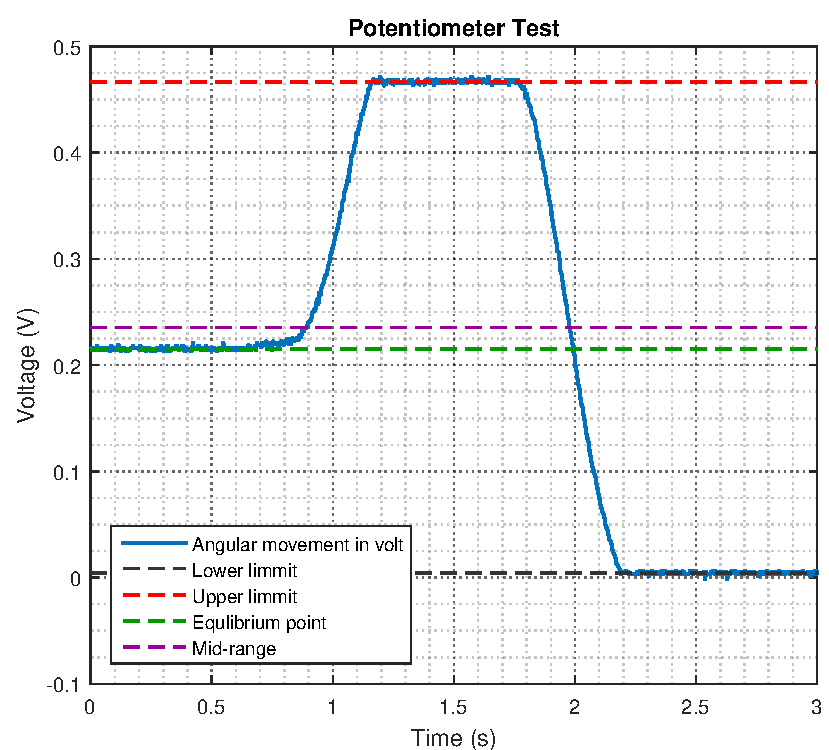
\includegraphics[scale=.5]{figures/PotentiometerResolution}
  			\centering
  			\captionsetup{justification=centering}
  			\captionof{figure}{\\Potentiometer measurements in volts}
  			\label{PotentiometerResolution}
  		\end{figure}\vspace{-5mm}
  	\end{minipage}
  	\hspace{0.03\linewidth}
  	\begin{minipage}{0.45\linewidth}
  		\begin{figure}[H]
  		%\vspace{.5cm}
  			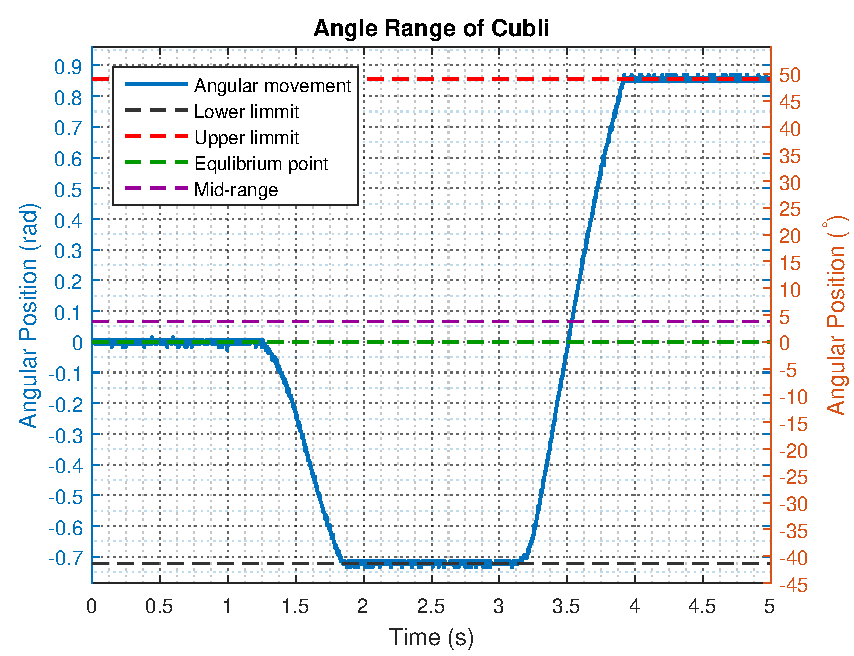
\includegraphics[scale=.5]{figures/PotentiometerResolutionDegRad}
  			\centering
  			\captionsetup{justification=centering}
  			\vspace{-.5cm}
  			\captionof{figure}{\\Potentiometer measurements converted to radians and degrees}
  			\label{PotentiometerResolutionRadDeg}
  		\end{figure}\vspace{-5mm}
  	\end{minipage}
\end{minipage}

The results of this test is shown above in \figref{PotentiometerResolution}, where the reference lines reveals an offset between the middle of the range and the equilibrium point of the Cubli frame.\\
This offset, also seen angle offset on \figref{PotentiometerResolutionRadDeg}, exists in the physical position of the frame. When the frame is standing it its equilibrium position it is displaces by approximately \si{3,9} degrees due to uneven distribution of mass around its center.\\
This results in a \si{48,9} degree range to one side of the optimal position and \si{41,1} degrees on the other\fxnote{STILL INVESTIGATING. IS NOT THAT UNEVEN AFTER ALL}.\\
To avoid complications it is chosen that the angle-offset must be accounted for such that the equilibrium position of the frame is at angle 0.


\subsection{IMU}
Acceleration is measured by the 3-axis accelerometer.

Angular velocity is measured by the 3-axis gyroscope. \fxnote{make a table with important info}

\subsubsection{Complementary filter}
A complementary filter is used to combine the measurement data from the accelerometer and gyros in the IMU. 
Data from the accelerometer is used to calculate an angle of the Cubli frame.
The gyroscope measurement is integrated to get the angle of the Cubli frame. Both measurements are done to find the change on the axis of movement of the Cubli.
The two angle measurements of the IMU are sent through a filter and then summed in order to get an angle of the Cubli frame. \fxnote{Make a proper sketch of the complementary filter, B}
\begin{figure}[H] 
	\centering
	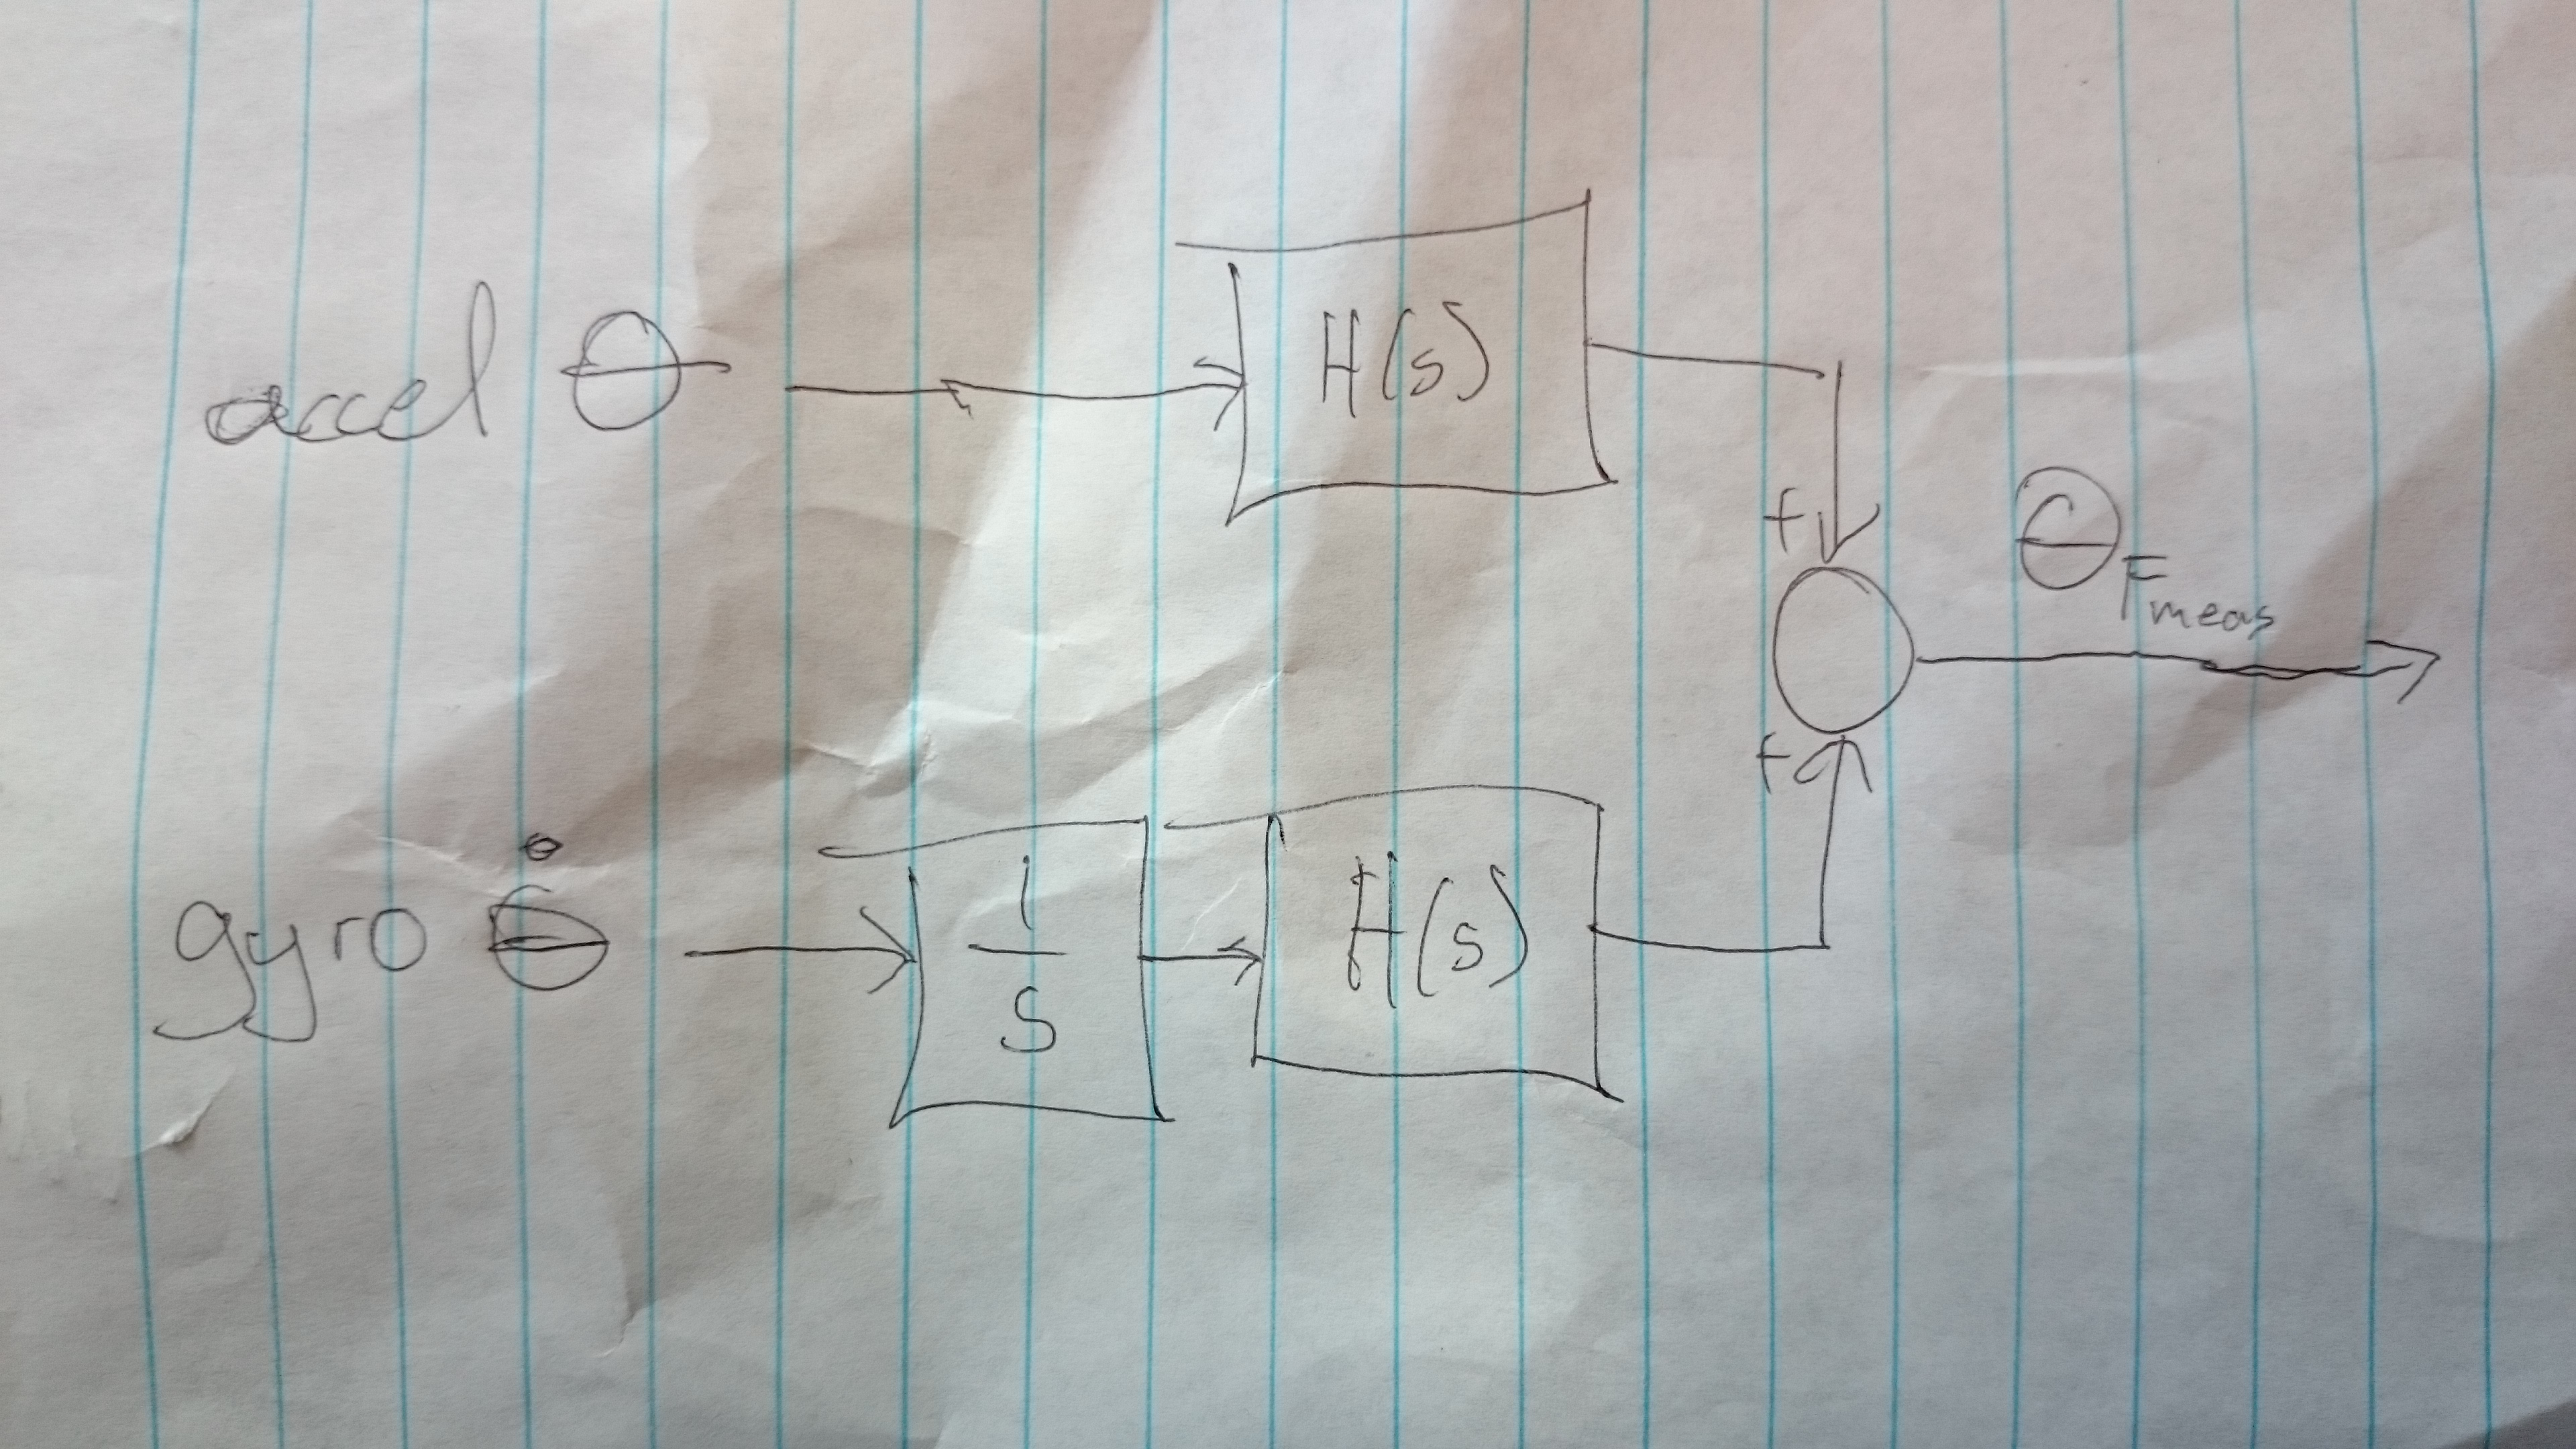
\includegraphics[scale=0.08]{figures/tempComplementaryFilter}
	\caption{Sketch of the structure of the complementary filter. Measurements from the accelerometer are calculated into an angle on the axis of movement. Data from gyro is used to find the angular velocity on the axis of movement}
	\label{blockComplementaryFilter}
\end{figure}
This is done to counteract drift of the gyroscope and error of the accelerometer.\fxnote{elaborate on the errors} 